\chapter{Dynamic Paralleotope Bundles}

In this chapter, we cover a method of generating template directions dynamically and automatically.
%
By dynamic, we mean that the template directions must be generated adaptively based on sampled trajectories and/or data from the state of the system.
%
By automatic, we mean that the template directions require no consideration from the user to proceed with the reachable set computation. This is in contrast to the original static algorithm treated in Section \ref{sec:static} where the user must input his or her own template directions to specify the parallelotopes before the computation begans.
%
To briefly outline the structure of this chapter, we first expound on two techniques we utilize to dynamically generate template directions at each step.
%
The first method is based on local linear approximations where the algorithm approximates the dynamics as a linear transformation based on sample trajectories.
%
The second method is based on Principal Component Analysis (PCA) where the algorithm runs the PCA procedure on the image points of the sample trajectories.
%
Finally, we cover the high-level pseudo-code of the dynamic algorithm and explain a set of parameters we feed into the algorithm in order to improve performance and the accuracy of the outputted reachable set.


%-----------------------------------------------------------------------------------------------------------------------------------------------------------------

\section{Drawbacks to the Static Algorithm}
Before we embark on introducing the dynamic algorithm, let us first consider a few motivating factors.
%
As discussed in Section \ref{sec:static}, the static algorithm requires template directions to be specified by the user in order for the reachable set computation to proceed.
%
The parallelotopes tended to be defined by a combination of axis-aligned directions or diagonal directions.
%
However, it is unclear whether these template directions work reasonably well over general non-linear dynamics.
%
This is a problem which has profound consequences for computing useful over-approximations.
%
Choosing the incorrect directions could very well lead to an over-approximation too conservative for any practical use.
%
Figure \ref{fig:bloat_cvdp} portrays a simple example of a reachable set whose wrapping error becomes explosive after a few steps.
%
In light of these ramifications, it is esstentially incumbent on the user to choose fruitful template directions that control the growth of the over-approximation.
%
Due to the inherent difficult nature of choosing these template directions, it may be unreasonable to delegate this responsibility to a practitioner who knows little about parallelotope-based reachability.
%
These drawbacks to the static algorithm motivate the rationale behind the \emph{automatic} aspect of our modified algorithm.

Additionally, as the template directions are set at the beginning before the reachable set computation proceeds, these directions cannot adapt to the dynamics as the computation executes.
%
There may be template directions which may yield much leaner over-approximations at an intermediate step during the computation.
%
Hence, the ability to change the composition of the parallelotope bundle by adding and removing parallelotopes based on a data-driven approach could yield leaner over-approximations.
%
These considerations motivate the rationale behind the \emph{dynamic} aspect of our modified algorithm.

\begin{figure}[t!]
\centering
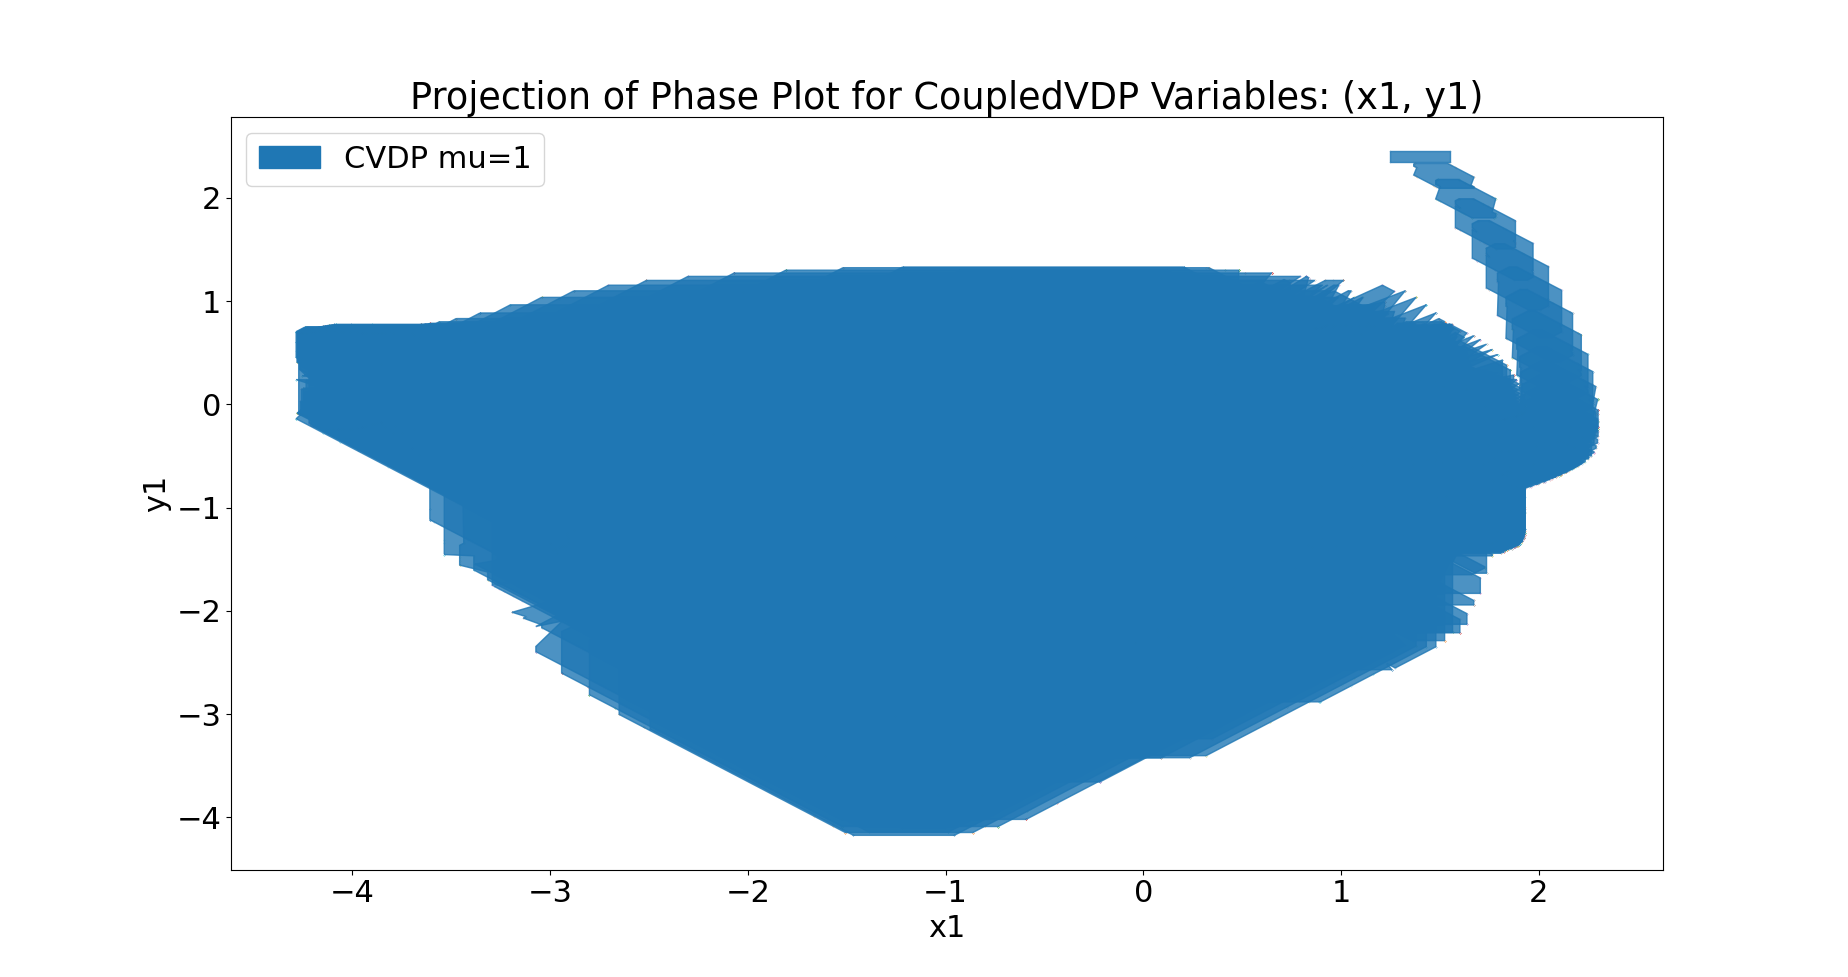
\includegraphics[width= 0.9\textwidth]{figures/cvdp20.png}
\caption{Consequences of choosing inappropriate template directions as demonstrated by the Coupled Vanderpol model. See Section \ref{sec:cvdp} for the model definition.}
\label{fig:bloat_cvdp}
\end{figure}

\section{Local Linear Approximations}
\label{sec:lin_app}
%
Intuitively speaking, if time step is discretized to be sufficiently small, propagating trajectories according to the non-linear dynamics $f$ for one time step could lead to good lienar approximations of the dynamics within a small region.
%
%
To do this, we first sample a set of points in the parallelotope bundle called \emph{support points} and propagate them to the next step using the dynamics $f$.
%
Support points are a subset of the vertices of the parallelotope that either maximize or minimize the template directions over the parallelotope bundle.
%
That is the support points are the set of points $P_{supp}$ defined as:
\begin{equation}
\label{eq:support}
 P_{supp} = \bigcup_{i=1}^n \{ \max_{x \in Q} \Lambda^Q_i\cdot x, \; \min_{x \in Q} \Lambda^Q_i\cdot x \}
\end{equation}
%
for all template directions of the bundle $\Lambda^Q_i$. We use the support points as a data-driven approach to determine the best-fit linear function to use. All points are found by a straightforward linear program.
%
%In this case, for small time steps a nonlinear function can be approximated fairly accurately by a linear transformation.
%
To find the approximate linear transformation, let $x_i$ denote the support points calculated by Equation \ref{eq:support}. We perform the following least-squares procedure: the objective would be to find an linear transformation $A$ such that it minimizes the following objective function:
\begin{equation}
  \label{eq:least_squares}
  \min_{A} \sum_{x_i} ||f(x_i) - Ax_i||^2_2
\end{equation}
%
where $||\cdot||_2$ is the standard Euclidean norm on $\reals^n$.
%
If the dynamics of a system are linear, i.e., $x^{+} = Ax$, the image of the parallelotope $c_{l} \leq \Lambda x \leq c_{u}$, is the set $c_{l} \leq \Lambda \cdot A^{-1} x \leq c_{u}$.
%
To see this, recall the constraint associated to the half-space representation (Definition \ref{def:halfspace_def} and Equation \ref{eq:halfspaceconst}). If we set our new template directions to be $\Lambda \cdot A^{-1}$, the image points of $A$ which satisfy the half-space constraint according to fixed offset vectors $c_l, c_u$ should be:
 \[ c_l \leq (\Lambda \cdot A^{-1})Ax \leq c_u \implies c_{l} \leq \Lambda x \leq c_{u} \]
%
This is satisfied by all the points defining parallelotope $P$ as desired. Therefore, the new template directions will exactly define the image of $P$ under linear dynamics. To exploit this property, given the template directions of the initial set as $\T_0$, we compute the local linear approximation of the non-linear dynamics and change the template directions by multiplying them with the inverse of the approximate linear dynamics.
%
%This will reflect the approximate template directions for one step forward. To continue to
%

%-----------------------------------------------------------------------------------------------------------------------------------------------------------------

\section{Principal Component Analysis}
\label{sec:pca}
The second technique for generating template directions performs Principal Component Analysis (PCA) over the images of the support points.
%
PCA is a standard technique in Statistical Machine Learning used to reduction of dimensionality by performing Singular Value Decomposition (SVD) on the covariance matrix generated by a set of data points.
%
Since the covariance matrix is symmetric by definition (i.e $A = A^T$), the eigenvectors of this matrix will always be a orthonormal basis of the system.
%
Using PCA is a reasonable choice as it produces orthonormal directions that can construct a rotated box for bounding the points.
%
% Give a very light sketch of the procedure here.
To compute the images of the trajectory points, the algorithm must first compute $P_{supp}$ and propagate them one step forward by the dynamics $f$. These image points fed into the PCA procedure.

%-----------------------------------------------------------------------------------------------------------------------------------------------------------------
\section{The Dynamic Algorithm}
\label{sec:dyna_algo}
Observe that in general, our input dynamics are non-linear and therefore, the reachable set is generally non-convex.
%
On the other hand, a parallelotope bundle is always a convex set.
%
To mitigate the drawbacks of this discrepancy, we can improve the accuracy of this representation by considering more template directions and more parallelotopes.
%
To this end, we add a parameter called \emph{template lifespan}, where we use the generated linear approximation and/or PCA template directions not only from the current step but also from previous steps.
%
During our benchmarks, we tune each of the options (PCA / linear approximation as well as lifespan option) to demonstrate that specific parameters generate more accurate reachable sets than those generated by the static algorithm presented in Algorithm \ref{alg:old}.

The new approach is given in Algorithm~\ref{alg:new}.
%
During each step, the algorithm computes a collection of template directions from the two techniques outlined in the previous two sections. The subroutines will be encoded as a subroutine labeled \texttt{ApproxLinearTrans} and \texttt{PCA} respectively.
%
The \texttt{ApproxLinearTrans} function computes the best linear approximation of the dynamics as specified in Section \ref{sec:lin_app}.
%
The \texttt{PCA} function returns a set of orthogonal directions using principal component analysis of a set of points as specified in Section \ref{sec:pca}.
%
Now each subroutine will return a collection of $n$ template directions, which in turn will specifiy exactly one parallelotope.
%
Hence, two parallelotopes, one generated by \texttt{ApproxLinearTrans} and the other by \texttt{PCA}, can be added to the parallelotope bundle at each step.
%

There are a few subtle points to be made about the sub-routines used in Algorithm \ref{alg:new}.
%
First, the algorithm makes use of helper function \texttt{hstack}, which attaches two matrices along their rows. In other words, \texttt{hstack} can be visualized as two matrices with the same number of columns stacked on top of one another.
%
Second, we assume that the sub-routine  \texttt{PCA} returns the orthonormal eigenvectors as rows. This assures that the eigenvectors are rows of a template direction matrix of a parallelotope.
%
Third, the \texttt{Maximize} and \texttt{Minimize} sub-routines encapsulate the linear programming procedures required to compute the support points as discussed in Equation \ref{eq:support}.
%
Both sub-routines take the feasible region as the first parameter and the objective function as the second parameter.
%
%The notation $M_{*,i}$ is used to refer to the $i^{th}$ column of matrix $M$.
 Finally, the subroutine \texttt{TransformBundle} is the same as specified in Algorithm~\ref{alg:old}.
%-----------------------------------------------------------------------------------------------------------------------------------------------------------------

\begin{figure}[t!]
\begin{algorithm}[H]
  \SetKwInput{KwInput}{Input}
  \SetKwInput{KwOutput}{Output}
  \SetKwFunction{CreatePCA}{CreatePCA}
  \SetKwFunction{CreateLin}{CreateLin}
  \SetKwFunction{TransformBund}{TransformBundle}
  \SetKwFunction{UpdateTemp}{UpdateTemplates}
  \SetKwFunction{GetSupp}{GetSupportPoints}
  \SetKwFunction{PropPoints}{PropagatePointsOneStep}
  \SetKwFunction{PCA}{PCA}
  \SetKwFunction{ApproxLinearTrans}{ApproxLinearTrans}
  \SetKwFunction{SetLifeSpan}{SetLifeSpan}
  \SetKwFunction{ExtractDirections}{ExtractDirections}
  \SetKwFunction{AddTemptoBund}{AddTemplateToBundle}
  \SetKwFunction{Maximize}{Maximize}
  \SetKwFunction{hstack}{hstack}
  \SetKwFunction{RemoveTemp}{RemoveTempFromBund}
  \SetKwProg{Fun}{Proc}{:}{}

\SetAlgoLined
\DontPrintSemicolon

\KwInput{Dynamics $f$, Initial Parallelotope $P_0$, Step Bound $S$, Lifespan Parameter $L$}
\KwOutput{Reachable Set Overapproximation $\overline\Theta_k$ at each step $k$}

$Q_0 \gets \{P_0 \}$ \;
$\Lambda^{accum} \gets I_n$ \tcp{Set to Identity Matrix} \;
% $\T_0 = \{ \{ P_0.\T_1, \ldots P_0.\T_n \} \}$ \;
$\Lambda^{Q_0} \gets \Lambda^{P_0}$ \tcp{Init Template Directions}

 \For{$k \gets 1$ \KwTo $S$}{
    $P_{supp} \gets $\GetSupp($Q_{k-1}$) (support points of $Q_{k-1}$) \;
    $P_{prop} \gets $ \PropPoints($P_{supp}$, $f$) (image of support points) \;

    $A \gets$  \ApproxLinearTrans($P_{supp}$, $P_{prop}$) \; \label{ln:linearapprox}
    $\Lambda^{accum} \gets \Lambda^{accum} \cdot A^{-1}$ \;
    $\Lambda_k^\text{lin} \gets \Lambda^{accum}$ \\ \; \label{ln:linapp}
    $\Lambda_k^\text{pca} \gets \PCA(P_{prop}) $\; \label{ln:pca}

    $\Lambda_k \gets \hstack(\Lambda_k^\text{lin}, \Lambda_k^\text{pca})$ \;
    $\Lambda^{total} \gets \Lambda_k$ \;
    \For{$i \gets 1$ \KwTo, $L$}{\tcp{If $L = 0$, then skip}
        $\Lambda^{total} \gets \hstack(\Lambda^{total}, \Lambda_{k-i})$
    } \;
    $Q_k \gets $ \TransformBund($f$, $Q_{k-1}, \Lambda_k$) \;
   $\overline\Theta_k \gets Q_k$ \;
 }
 \Return{$\overline\Theta_1 \ldots \overline\Theta_S$} \;
 %
 \;
   \Fun{\GetSupp{$Q$}}{
     $P_{supp} \gets \emptyset$ \;
      \For{$P \in \ptopeset{Q}$}{
        \For{$i \gets 1$ \KwTo $n$}{
         $P_{supp} \gets P_{supp} \cup ~ \Maximize (Q, \Lambda_i^P) \cup ~ \Maximize (Q, -\Lambda_i^P)$
        }
     }

  \Return{$P_{supp}$}
  }
\end{algorithm}
\caption{The Automatic, Dynamic Reachability Algorithm}
 \label{alg:new}
\end{figure}

%-----------------------------------------------------------------------------------------------------------------------------------------------------------------

Algorithm~\ref{alg:new} computes the dynamic templates for each time step $k$.
%
Line~\ref{ln:linearapprox} computes the linear approximation of the non-linear dynamics and this approximation is used to compute the new template directions according to this linear transformation in Line~\ref{ln:linapp}.
%
The PCA directions of the images of support points is computed in Line~\ref{ln:pca}.
%
For the time step $k$, the linear approximation and PCA templates direction matrices are given as $\Lambda_{k}^{lin}$ and $\Lambda_{k}^{pca}$, respectively.
%
To improve the accuracy of the reachable set, we compute the over-approximation of the reachable set with respect to not just the template directions at the current step, but with respect to other template directions for time steps that are within the template lifespan parameter $L$.
%
Alternatively, we assign each parallelotope a parameter $L$ which dictates the number of steps we keep the parallelotope in the bundle after adding it in the current step.
